\documentclass[0-thesis.tex]{subfiles}

\begin{document}
This thesis proposes an update architecture based on SUIT. The architecture is technology
agnostic and adds on top of SUIT tokens and certificates for identifying and authorizing
actors, a life cycle perspective on device management, and defines what information is
needed for a device to take part of an update procedure. Furthermore the thesis presents
profiles for the architecture which implementers can use, these are introduced in Chapter
\ref{chap:profiles}. Five key areas that the architecture must define have been
identified:

\begin{itemize}
    \item Roles of devices, servers, and operators
    \item Key management of IoT update procedure
    \item Device profiles and communication
    \item Update authorization
    \item Update handling for local upgrades
\end{itemize}

\begin{figure}
    \caption{Example workflow of an update procedure.}
    \label{fig:communication-workflow}
    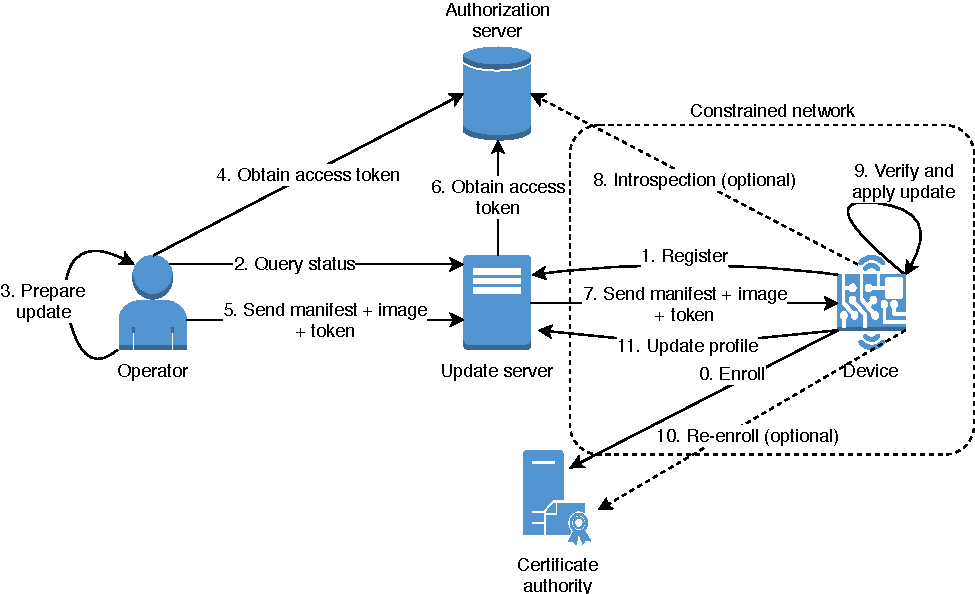
\includegraphics{images/update-flow.pdf}
\end{figure}

By putting the five key areas together, Figure~\ref{fig:communication-workflow} shows an
example update flow in the architecture. Note that where the SUIT standard would
differentiate between the author of an update and an operators, this architecture will for
simplicity regard them as the same actor. For the same reason, the architecture will not
differentiate between device and network operators. An operator is an actor that tracks
device statuses and prepares, signs, and sends updates to devices.
Figure~\ref{fig:communication-workflow} gives a brief introduction to the concepts needed
to understand the architecture, these concepts will be explained in more detail throughout
sections \ref{sec:roles}-\ref{sec:authorization}. In this particular example the update
procedure is initiated by the operator by querying the server for device status and then
pushing an update. The manifest and image are distributed together. The steps can be
briefly explained as:

\begin{enumerate}
    \setcounter{enumi}{-1}
    \item The device enrolls at the CA and receives a certificate.
    \item The device registers at the server which now holds a profile for the device.
    \item The operator queries the server for device status in order to prepare an update.
    \item The operator prepares a manifest and image and signs them.
    \item The operator requests an authorization token from the authorization server in
            order to gain access to applying the update.
    \item The signed manifest and image are sent to the server with the authorization
            token.
    \item The server requests an authorization token from the authorization server in
            order to gain access to applying the update.
    \item The signed manifest and image are sent with the server's authorization token to
            the device.
    \item The device requests introspection data from the authorization server
            to verify the authorization token. This step is optional.
    \item The device decrypts and verifies the manifest and image and applies the update.
    \item The device's certificate broke as part of the update and it uses a new
            pre-shared key included in the updated image to re-enroll. This step is
            optional.
    \item The device updates its profile at the server by re-registering.
\end{enumerate}

Section~\ref{sec:roles} defines what a device, server, and operator means in the context
of the update architecture. Section~\ref{sec:key-management} discusses what is needed for
devices to enroll in a PKI and how keys are handled during updates.
Section~\ref{sec:communication} describes how devices, servers, and operators can
communicate and shows an example workflow of communicating an update.
Section~\ref{sec:authorization} describes the purpose of issuing authorization tokens, how
devices can use them, and who is to be authorized. Section~\ref{sec:upgrading} discusses
different means of handling the payload when applying an update.
Finally Section~\ref{ssec:use-cases-examples-topologies} shows the architecture applied to
different use cases.

\section{Roles of Devices, Servers, and Operators}
\label{sec:roles}
This section explains the notion of devices, servers, and operators in the architecture,
their responsibilities, and their functionality. Section~\ref{ssec:what-is-a-server}
covers the topic of servers, Section~\ref{ssec:what-is-an-operator} covers operators, and
Section~\ref{ssec:what-is-a-device} briefly covers devices.

\subsection{What Is a Device and What Do They Do?}
\label{ssec:what-is-a-device}
Devices are constrained, low-power IoT appliances connected to a constrained network. They
are running the applications of the network and performs simple tasks such as measurement
using sensors. The devices communicate wirelessly and must be secured from attackers while
being able to be updated. They communicate with each other, servers, and operators.

Communication with servers and operators requires the servers and operators know how to
reach the devices if they want to initiate contact. Devices must thus register profiles at
servers, and must be enrolled in order to be trusted. In order to register a profile at a
server, the server must offer an API that allows a device to POST its information
(vendor and class ID as well as version) to the server. 

Devices have to trust servers and operators wanting to send them updates. In order to do
so, devices need predetermined whitelists of servers and operators. The identity of a
server or operator can be checked using certificates and by then matching against the
whitelists, communication can be allowed or prohibited. Servers and operators that are
whitelisted still need to be authorized to perform an update, this is discussed further in
Section~\ref{sec:authorization}.

To properly handle updates a device needs a local update handler. The update handler is
responsible for decrypting manifests and images, parsing and verifying the manifest, and
preparing the image for boot. How and where the device stores manifest and image is
discussed in further detail in Section~\ref{sec:upgrading}.

\subsection{What Is a Server and What Do They Do?}
\label{ssec:what-is-a-server}
Servers are responsible for transporting manifests and images to the devices, acting as
image repositories, and keeping track of device profiles. After enrollment devices
register at a server and the server creates a profile for that device. The profile
contains the vendor and class IDs and firmware version of the device. This allows the
server to know through which protocols the device can be contacted and which version it
should be updated to. Operators, discussed in the next section, send signed manifests and
images to servers, and can query them for device status.

Devices should contain a list of servers and by trusting the certificate authority they
can validate server certificates. A server is thus any machine that is enrolled, has a
valid certificate, and is included in the device's list of servers. The reasoning behind
this definition is that a standard solution for updates should not assume the topology of
an IoT network. The server may be a machine acting as a proxy between a traditional
network containing the operator and a constrained network with IoT devices. The server
could be a more capable IoT device located entirely within the constrained network and be
contacted through a proxy. The server could be located entirely within the traditional
network and use a proxy to communicate with devices of the constrained network.
Section~\ref{sec:use-cases-examples-topologies} shows different use cases, highlighting
this aspect.

A server must provide an API for a device to register, this can be done by letting the
device POST vendor and class IDs and version to some endpoint. Furthermore devices must be
able to pull updates from the server, this also requires some API the device can use for
querying. Furthermore operators will also be querying the server for statuses of devices.
This functionality can be more fleshed out as it interacts with a human, and can offer
functions for retrieving statuses of devices from a certain vendor or class, or devices
running a certain firmware version. Allowing the operator to filter devices in the network
while querying is important as IoT networks can contain a large amount of devices, and it
is imperative to find the ones in critical need of updates first.

% TODO: Does a device need one keypair for each server? Does it need one keypair for all servers?
A device can be aware of several servers, and different devices can be mapped to different
servers. This can make device management easier as certain classes of devices can be
handled by certain servers. By allowing a device to receive updates from several servers,
the update mechanism architecture also displays a form of robustness. If one server is for
instance located entirely within the constrained network and the connection between that
server and the operator is severed, updates can still be distributed through other
servers. If devices are pulling updates, they can query the servers in order of their list
of servers. If updates are pushed, devices keep the connection with the server pushing the
update.

Which machines are allowed to act like servers can be boiled down to a few important
points no matter the topology of choice:

\begin{itemize}
    \item The server is enrolled and has a valid certificate
    \item The server is included in a device's list of servers
    \item The server can request authorization tokens and be authorized to update a device
    \item An operator can reach the server and is authorized by the server to query device
            status and upload updates
\end{itemize}

\subsection{What Is an Operator and What Do They Do?}
\label{ssec:what-is-an-operator}
% TODO: Operators need a way of creating manifests, querying servers, and using the
% queried device profiles to send updates either directly or through the server.
Operators are people authorized to upload manifests and images to a server. They can also
optionally upload manifests directly to a device depending on the architecture. Operators
prepare manifests and images, signs and transports them with an authorization token to a
server, which then forwards them to a device. The signing ensures end-to-end security for
images and manifests between operators and devices. Authorization is further discussed in
Section~\ref{sec:authorization}.

Like a list of servers introduced in Section~\ref{ssec:what-is-a-server}, devices also
need a list of operators. This is because if an operator wishes to send a manifest
directly to a device, the device needs to be aware of the operator and permit traffic from
that operator. Just like with mapping devices to servers, devices can receive manifests
from several operators and different devices may interact with different operators. This
creates opportunities to logically divide a network between different operators. An
example use case is a constrained network supported by different vendors where the
respective vendors should only be able to service their respective devices. It can also
create a hierarchy, where certain operators may directly interact with devices but other
operators must interact with devices through servers. Yet again the point is to prepare
for as many different scenarios as possible and create a flexible architecture.

As with servers, the essence of being an operator can be captured in a few points:

\begin{itemize}
    \item An operator is enrolled and has a valid certificate
    \item An operator is included in a device's list of operators (and therefore can send
            manifests to the device)
    \item An operator is trusted by a server to send manifests and images to the server
\end{itemize}

\section{Key Management of IoT Update Procedure}
\label{sec:key-management}
% TODO: Consider updates breaking certificates. Why would they? Lack of understanding concerning
% certificates perhaps
% Two pairs of keys from one PSK? Are two pairs needed?
The architecture will, in order to align with the goals of SUIT, be based on asymmetric
cryptography. The availability of EST-coaps makes this feasible in IoT contexts but other
enrollment protocols could also be used. This means a \gls{ca} is needed to act as a
trusted third party distributing certificates. The certificates are linked to a public key
which has a private key partner and are used to verify the correctness of a public key.
Certificates are signed by the CA and in order to trust them, device have to trust the CA
itself.

In order to enroll, a pre-shared key is proposed. This is the approach used in EST-coaps,
but it is not chosen for that reason. If a pre-shared key is not used the CA cannot be
sure the device asking to enroll really should be part of the trusted network. If an
attacker obtains a valid certificate they could communicate with devices and servers alike
and no one would be able to tell it is a malicious actor. CAs must know they are issuing
certificates to the correct devices and pre-shared keys gives devices a means of
identifying themselves. Pre-shared keys could be used for encrypting all traffic but as
they are less scalable and harder to manage than certificates, they are just used for
enrolling.

A device that is enrolling has to trust the CA issuing the certificate. If it cannot do
so, how could it know it received a valid certificate? An attacker would love for a device
to use the attacker's public key instead, and if an attacker poses as a CA it could issue a
certificate with its own public key and then sign it. In order to trust the CA, a device
needs to have the certificate of the CA it is enrolling with or some other CA further down
the chain of trust. By verifying the signature on the newly enrolled certificate with the
CAs own certificate, a device can be certain they are using the correct keys.

When applying updates, certificates might not be valid anymore. This is implementation
dependant and might not always be a problem, but the architecture should be prepared for
these situations. In the case an update breaks a certificate, the certificate cannot be
used for communication and thus the device cannot use it to re-enroll either. In this
case, a new pre-shared key should be part of the update so that the device can enroll as
if it was factory new. The process of issuing pre-shared keys might be difficult to
automate as the CA must be aware of which keys to accept, but it is needed to ensure the
security of future device communication.

\section{Device Profiles and Communication}
\label{sec:communication}
In heterogeneous networks of IoT devices, each device might sport a specific protocol
stack. In order to enable different devices to be updated, servers must be aware of how to
reach these devices. This problem introduces the notion of device profiles containing
information about device capabilities and software versions. 

When devices have enrolled and obtained a valid certificate, they must contact their
respective servers so the servers can create profiles of the devices. The profiles will
tell through which protocols to reach a device and what software versions the device is
using. In order to achieve this, devices must first know which servers to contact. This
can be solved through shipping devices with a list of servers. This list can later on be
updated like any other software. Furthermore, the devices use vendor and class IDs as
described in the SUIT information model. The information model uses these pieces of
information to verify an update is intended for a specific device by matching the IDs, but
they can also be sent to a server to tell it what kind of device is contacting it. The
server can infer a profile based on the IDs it is sent, or simply use the protocols the
device chose to contact it. The devices also need to be aware of how to register, for
instance by POSTing to a specific server endpoint. 

When updating there are possibilities regarding how the updating process is initiated. An
operator can query the server for the status of one or several devices, prepare an update
for them, and have the update pushed through the server. Optionally the operator could
send a manifest to the device explaining when the update is to be applied and put the
image on the server. Later when the device should update, the device pulls the image from
the server, validates it using the already received manifest, and updates. Both the pull
and push approaches assume the devices are already enrolled and registered at the server.

After updating, the device's capabilities might have changed, for instance by having a new
protocol implemented in software. The version has also changed due to applying an update.
After an update, a device should notify all its servers so they can update the device
profile (or simply discard the old one and generate a new, as if the device registered for
the first time). This ensures the servers view of the devices is up to date and that
communication will always happen through the intended and supported protocols. The
functionality of registering is the same as when a device is new and thus not costly to
implement.

There are alternatives to using device profiles. One alternative is to instead keep a list
of known protocols implemented by devices in the network, and when pushing updates to a
device trying each protocol in sequence. This has the benefit of not needing to keep and
continuously update profiles, but also has some issues. One issue is that you still need
to keep some state of the devices on the server regarding firmware version. If the server
does not know what the status of device versions are, it cannot help a human operator
decide about deploying updates. 

Another drawback is that devices might implement common protocols but have different
preferences. If two devices implement some common protocols but one of them supports
hardware operations for encrypting one of the protocols, it will prefer using that
protocol with the server, whereas the other device might not. The server will however,
without information about device preference, try the same sequence of protocols with both
devices.

Furthermore, as communication can be unreliable over these networks, the server
cannot know for sure if a device does not respond due to not understanding the protocol
and therefore dropping the packets, or if the response just got lost in transmission. It
is more robust to keep track of which protocols devices support and conform to the
preferences of the constrained devices.

Lastly, instead of using profiles all communication could be initiated from the device
side, meaning updates are only done through a pulling mechanism. This would not enable the
use case of pushing updates which could be critical if a vulnerability must be patched
right away. Operators must be given the choice to push updates to their devices, and thus
servers must be able to initiate contact with devices.

\section{Update Procedure Authorization}
\label{sec:authorization}
% TODO: Discuss the 4 different kinds of tokens, when they are used, and why. When talking
% about who needs to authorize [try to] explain the issues with proof-of-possession keys
% and verifying the holder of the key when forwarding messages and that it does not work.
% Instead introduce a token per hop.
A flexible architecture enables different configurations of servers, operators, and
devices. An operator might be authorized to update all parts of all devices, or be
constrained to updating a specific piece of functionality for a subset of the devices.
Operating system vendors might be allowed to push security updates for the operating
system but not change the application code. Controlling access rights is a security issue
and the architecture must support it.

How clients can access a protected resource through authorization tokens is described in
\parencite{ace} and Figure \ref{fig:ace-flow} shows an adaptation of the protocol flow
from that document. The figure shows a client wanting to access a resource requesting a
token from an authorization server. The token is returned to the client, which can then
send a request with the token to the server holding the resource. If necessary, the
resource server can send an introspection request to the authorization server asking for
more information about the token in order to verify it. If everything goes as planned, the
client is allowed the resource.

\begin{figure}
    \caption{The protocol flow of ACE. Adapted from \parencite{ace}.}
    \label{fig:ace-flow}
    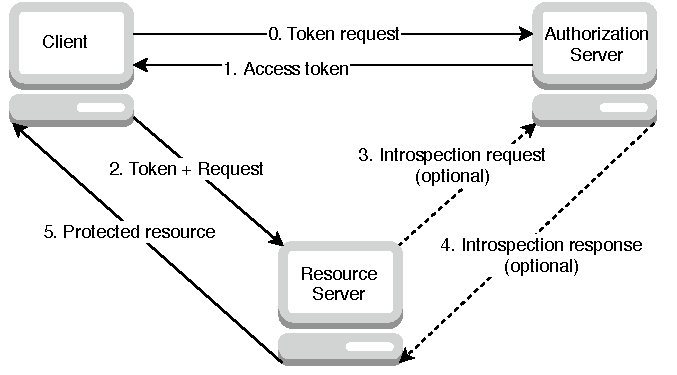
\includegraphics{images/ace.pdf}
\end{figure}

In the context of the update architecture, the client would be a party needing to
authorize themselves, i.e. an operator or server. The access token would have to be of a
lightweight variant since they are to be used on constrained devices, but which variant is
implementation specific. Tokens will be sent with updates (signed manifests and images) to
devices and the resource sought for is the ability to update the device. The device will
thus not respond with a particular resource, but instead if the token is valid recognize
the originator of the update as an authorized one and proceed with the update.
Introspection is an interesting feature of ACE since it requires less from the device
concerning validating tokens. Instead of doing everything on its own, the device can ask
the server for additional information making the validation procedure easier. This however
requires some extra communication which is power consuming for an IoT device. To use
introspection or not is yet again an implementation issue, but authorization servers
should be both enrolled and reachable for devices to send introspection requests if
necessary.

Who is supposed to authorize? As updates will be sent from operators through servers to
devices, the devices need to know the originator of an update is authorized to issue the
update. The proposition is to only require operators to authorize. No matter how updates
are initiated or distributed (pull vs push and manifest and image together vs separately),
updates at some point must be crafted, signed, and sent by an operator. The operator is
making the decisions about updating, and thus must authorize these decisions through
tokens. Servers deliver the updates to devices, but do so as a relay for operators as
well as acting as repositories for images and device profiles. The messages forwarded by
servers will contain the authorization token granted to an operator. This token can in
addition to authorizing the update on a device be used by the server to authorize the
usage of the server by the operator. 

Not requiring servers to authorize should not pose any issues as the update must always be
prepared in a previous step by an operator that authorizes. Also, it makes the flow of
applying an update easier by not needing and update server to communicate with an
authorization server. Requiring update servers to authorize would not add any security to
the devices as the update already will be shipped with a token authorizing the update.

\section{Update Handling for Local Upgrades}
\label{sec:upgrading}
% TODO: How to handle decryption and validation
% I like the idea of decrypting once and storing decrypted image with its hash for smaller
% bootloader procedure. Implementation specific though
% Cite mailing list perhaps?
% What happens locally + example update flow
When an update has finally arrived to the device, it must be processed and then installed.
The process of decrypting, verifying, and installing the image is heavily implementation
specific with most of the details being out of scope for the architecture. However, since
devices operate using different hardware and bootloaders they must be given the freedom to
update in the way that makes most sense for them and the architecture should support this
while requiring the approach is secure.

By including optional fields such as decryption instructions, processing steps, and
postconditions in the manifest, update handlers and bootloaders can take care of updates
in various ways. This enables different ways of applying updates within the same
architecture. What the update handlers and bootloaders of all devices have in common is
that they must trust the source of the update, they must be able to decrypt the update,
they must be able to verify the validity of the update, and they must be able to do this
safely such that an unexpected power cycle does not brick the entire device.

Still being in the realm of very constrained devices, the bootloader should be as simple
as possible. This is also a requirement stated by SUIT on the architecture. By decrypting
and verifying the image at every boot the boot procedure will be secure but quite complex.
Also if a power cycle occurs during image decryption, the device might not be able to
recover. Decrypting the image as part of the update mechanism and writing it unencrypted
to flash would allow for a simpler bootloader, but is less secure as the device would boot
from an unencrypted image.

By storing the manifest containing the image digest, unencrypted images can be verified by
comparing their digest to the one in the manifest. Calculating a digest is less demanding
than decryption, and a power cycle would just interrupt the digest calculation instead of
the decryption of the actual bootable image. In order to make sure the manifest is correct
upon boot, the digest of the manifest can be calculated and stored alongside the manifest
and image. Optionally the manifest can be encrypted instead as it typically will be much
smaller than the image, but again a power cycle during decryption could lead to undefined
behavior.

In addition to storing the manifest for verification upon boot, the manifest also has to
be stored in order to prevent rollback attacks. It contains monotonically increasing
sequence numbers to ensure devices do not install older, possibly vulnerable images, but
in order to compare sequence numbers the most recent manifest has to be kept around.
Manifests should be kept for the update handler to compare sequence numbers, and for the
bootloader to verify images.

\section{Use Cases and Example Topologies}
\label{sec:use-cases-examples-topologies}
As discussed, operators, servers, and devices can interact in many ways. The architecture
tries to be flexible allowing for different network topologies and configurations. The
important parts are that devices can enroll and register, all actors have valid
certificates, and that updates can be authorized. The following examples all assume
devices are in the maintenance stage of the life cycle, and re-enrollment and updating
profiles are omitted to make the figures clearer.

% TODO: Rewrite use cases, completely new figures
Figure~\ref{fig:elderly-home} shows an example architecture with one operator, one
update server, one authorization server, and one device. The operator is capable of
running the protocols needed to communicate in the constrained network, and can thus
interact directly with both the device to send manifests and server to send images. An
architecture like this allows for servers to be distributed within the constrained
network, possibly as more capable IoT devices.

\begin{figure}
    \caption{An operator communicating directly with machines in the constrained network.}
    \label{fig:elderly-home}
    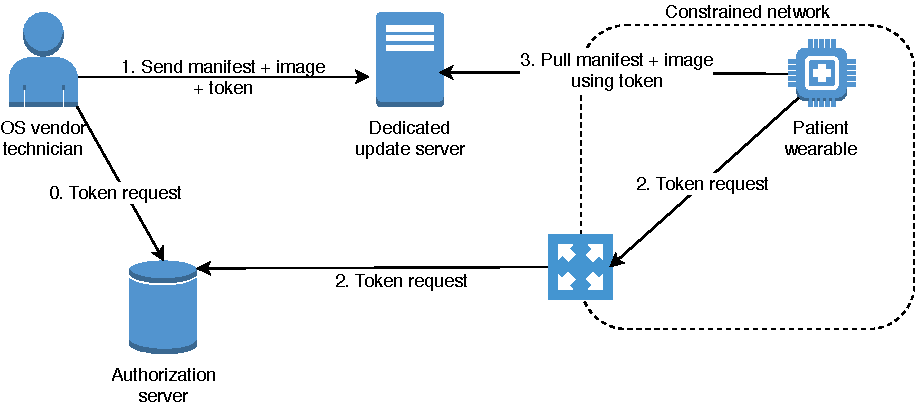
\includegraphics{images/use-case-elderly-home.pdf}
\end{figure}

Figure~\ref{fig:smart-home} shows an operator sending updates entirely through an
update server. The update server is located outside the constrained network and acts as an
proxy for the operator to reach the devices. The update is distributed from the server to
two devices, where one device accepts the update and the other rejects the update since
the operator was not authorized to apply it to that device.

\begin{figure}
    \caption{An operator communicating with an update server that pushes the update to two
                devices, with one device rejecting it.}
    \label{fig:smart-home}
    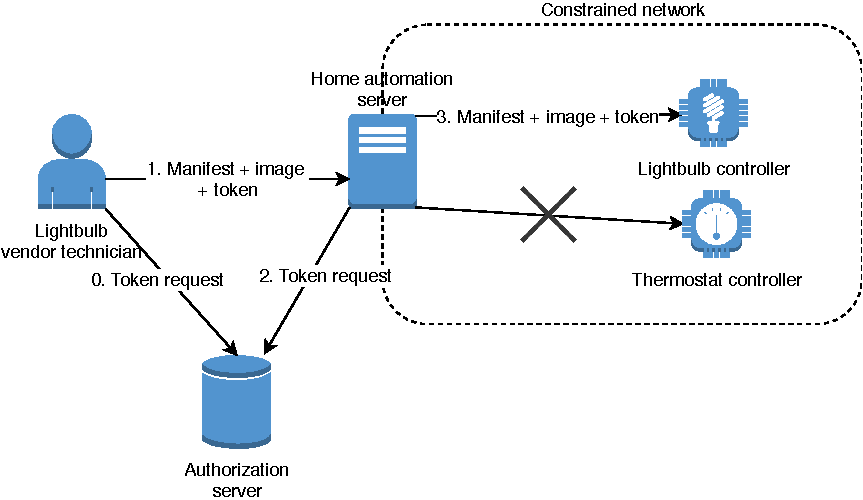
\includegraphics{images/use-case-smart-home.pdf}
\end{figure}

Figure~\ref{fig:industry} shows a more elaborate topology. It contains one
operator, one authorization server, two update servers, two devices, and a proxy. The
update is distributed to both servers, each server forwarding the update to one device
each. The first device accepts and applies the update. The second device requires more
information about the authorization token, and thus sends an introspection request. The
authorization server is located outside the constrained network, and the introspection
request must go through a proxy in order to reach it.

\begin{figure}
    \caption{An operator pushes updates to two servers forwarding it to one device each. 
                One device perform an introspection request to validate the authorization 
                token.}
    \label{fig:industry}
    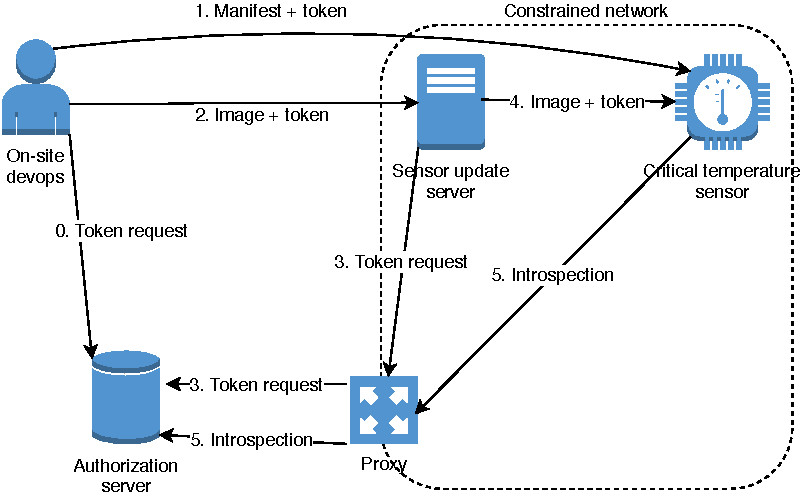
\includegraphics{images/use-case-industry.pdf}
\end{figure}

What these three examples have in common is that the operator always resides outside the
constrained network, devices always reside within the constrained network, and that
servers transport updates to devices alongside authorization tokens. Since operators
reside in traditional networks using traditional protocols such as HTTP over TCP, a proxy
mechanism may be necessary to communicate with the often UDP based constrained networks.
The update server can act as a proxy, or a dedicated proxy could be used. If the operator
has the proper protocols implemented, they could communicate manifests directly to a
device.

\end{document}